%----------------------------------------------------------------------------------------
%	PAKET-/ UND ANDERE DOKUMENT-IMPORTS
%----------------------------------------------------------------------------------------
\documentclass{scrartcl}   % Formateinstellungen
\usepackage[ngerman]{babel} % deutsche Silbentrennung
\usepackage[utf8]{inputenc} % deutsche Umlaute
\usepackage{placeins}   % verbessert Anzeige eines Floats hinter dem Befehl \FloatBarrier
\usepackage{amsfonts}   % neue Schriftanpassungen (wird von amssymb (s.u.) geladen)
\usepackage{amssymb}    % erweitert Benutzung von amsfonts (s.o.)
\usepackage{amsmath}    % Vielzahl von neuen mathematischen Umgebungen und Befehlen (wird von mathtools (s.u.) geladen)
\usepackage{mathtools}  % Verbesserung von amsmath (s.o.)
\usepackage{booktabs}   % Tabellen ohne vertikale Striche
\usepackage{siunitx}    % Einheitensystem
\usepackage[margin={0.3cm,0.3cm},font=singlespacing,labelfont=bf,labelsep=endash]{caption} % Bildunterschriften
\usepackage{wrapfig}    % Bild von Text umfließen lassen
\usepackage{sidecap}    % ermöglicht Überschriften neben Bildern / Tabellen
\usepackage{setspace}   % zum Definieren des Zeilenabstandes
\usepackage{eurosym}    % ergänzt optimales Euro-Zeichen
\usepackage[perpage,marginal]{footmisc} % ermöglicht Fußnoten und das Verändern dieser
\usepackage{graphicx}   % ermöglicht besseres Einbinden von Grafiken
\usepackage{fancyhdr}   % zum Erstellen von Kopf- und Fußzeilen
\usepackage{listings}   % ermöglicht Quellcodelisting
\usepackage{color}  % Farb-Management von Vorder- und Hintergrundfarben
\usepackage{pdfpages}   % ermöglicht das Einbinden von ganzen oder nur Teilen von PDFs
\usepackage{lineno} % Zeilenzählung
\usepackage{framed} % ermöglicht das Einrahmen von Elementen
\usepackage{pifont} % fügt Symbol-Schriften hinzu
\usepackage[hidelinks]{hyperref}    % ermöglicht das Hinzufügen von Links und Verweisen innerhalb
                                    % des PDF Dokuments und weitere Einstellungen
\usepackage[left=2.5cm,right=2cm,top=2cm,bottom=2cm,includeheadfoot]{geometry}  % Größenanpassung der Seite
%----------------------------------------------------------------------------------------


%----------------------------------------------------------------------------------------
%   KONFIGURATIONEN
%----------------------------------------------------------------------------------------
\begin{document}
\setlength{\parskip}{1ex}   % Abstand zwischen Absätzen 
\parindent 0pt  % legt Einrücke der ersten Zeile fest
\renewcommand{\thefigure}{\arabic{figure}.\alph{ab}}    % Umdefinieren von Bildnummern

\definecolor{darkblue}{rgb}{0,0,.6} % Festlegen der Farben
\definecolor{darkred}{rgb}{.6,0,0}  % Festlegen der Farben
\definecolor{darkgreen}{rgb}{0,.6,0}    % Festlegen der Farben
\definecolor{red}{rgb}{.98,0,0} % Festlegen der Farben

\lstloadlanguages{Java} % lädt Programmiersprachen
\lstset{language=Java,basicstyle=\footnotesize\ttfamily,commentstyle=\itshape\color{darkgreen},keywordstyle=\bfseries\color{darkblue},stringstyle=\color{darkred},tabsize=3,showspaces=false,showtabs=false,columns=fixed,numbers=left,frame=single,numberstyle=\tiny,breaklines=true,showstringspaces=false,xleftmargin=1cm} % Erstellen eines Codeblocks
    
\pagestyle{fancy}   % Setzen des Seitenstyles "fancy" ermöglicht eigenes Erstellen einer Kopf- und Fußzeile
\fancyhf{}  % alle Kopf- und Fußzeilenfelder bereinigen
\fancyhead[L]{\leftmark}    % Kopfzeile links (mit "leftmark" erstellt man im Header das Chapter, mit "rightmark" die Section)
\fancyhead[C]{} % zentrierte Kopfzeile
\fancyhead[R]{\thepage} % Kopfzeile rechts
\fancypagestyle{plain}  % legt Seiten-Typen fest

\newcommand{\barrow}{\item[\ding{228}]} % hinzufügen des Pfeil-Aufzählsymbols unter dem Command \barrow
%----------------------------------------------------------------------------------------


%----------------------------------------------------------------------------------------
%   1. SEITE
%----------------------------------------------------------------------------------------
\titlehead{\Large

\begin{center}
\begin{framed}
\centering {Inoffizielle Lösungen und Erklärungen - \href{https://www.inf-schule.de/inf-schule}{inf-schule\textsuperscript{\textcopyright}} (\href{https://creativecommons.org/licenses/by-sa/4.0/legalcode.de}{\textit{Lizenz}})}

\centering {\Large\textbf{\href{https://inf-schule.de/testKapitel}{0.0 Test-Kapitel}}}
\end{framed}
\end{center}}

\title{\huge{\href{https://inf-schule.de/testThema}{1.1\\Test-Thema}}\\
\vspace{0.5cm}
\begin{figure}[ht]
	\centering
	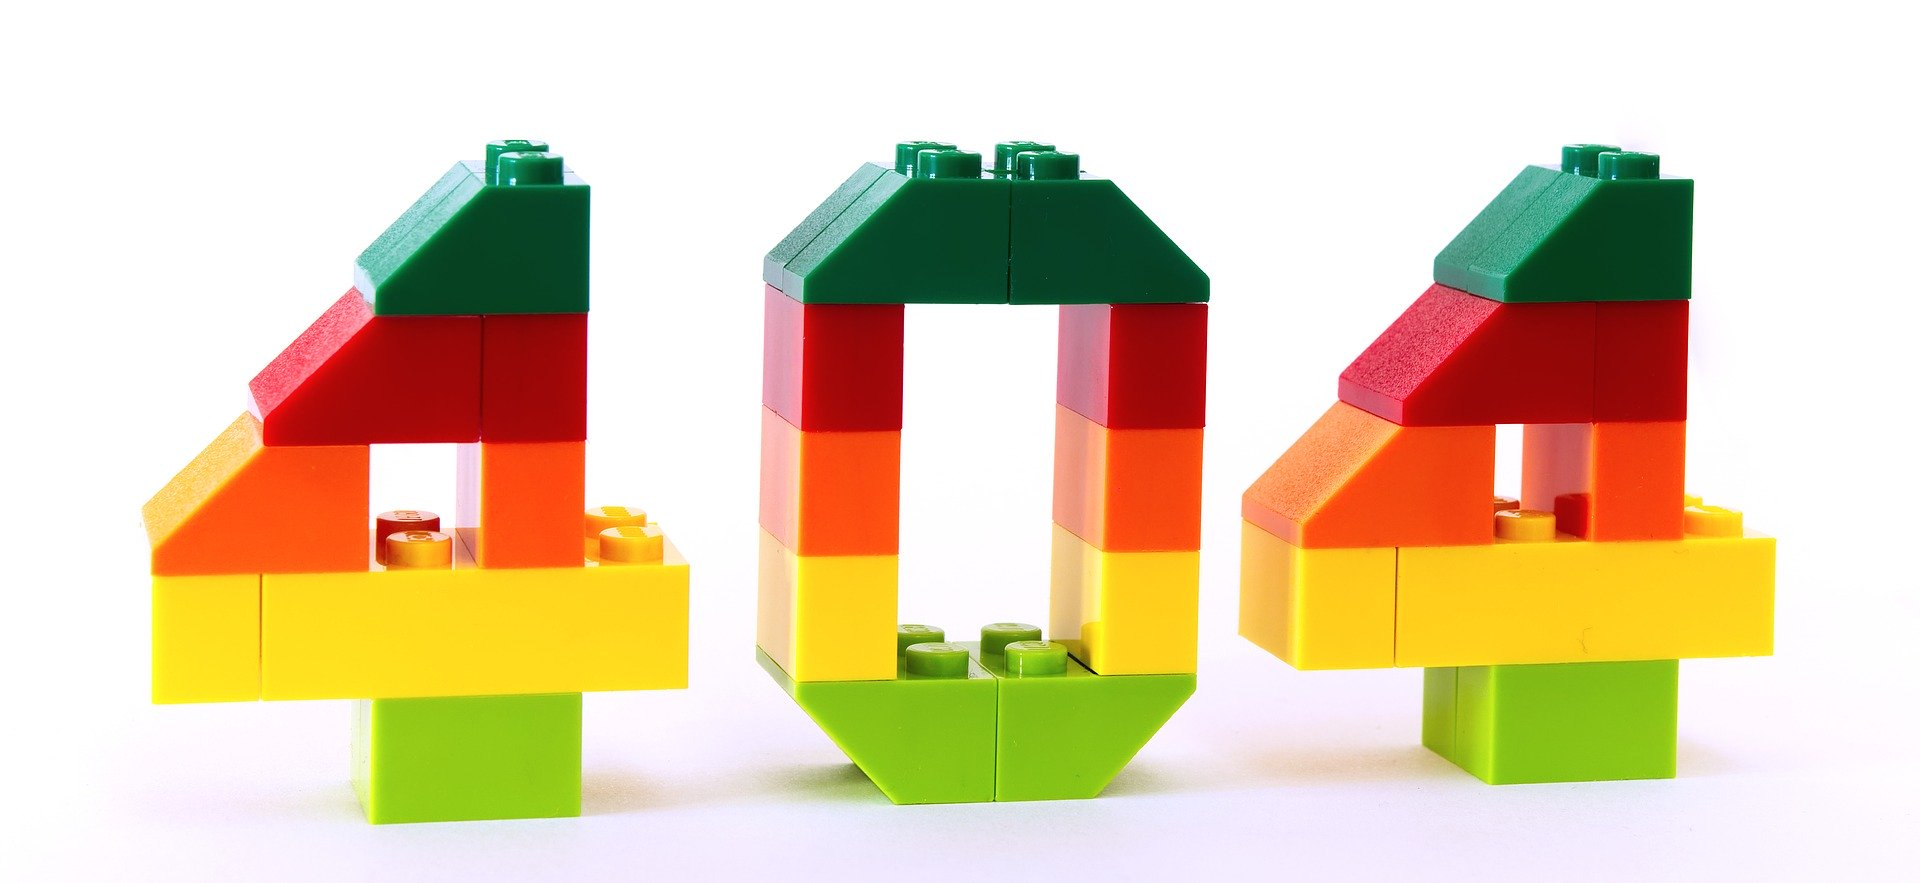
\includegraphics[height=4.5cm]{Template/template.png}
\end{figure}
\vspace{2cm}}

\author{\textbf{Benötigte IDEs:}\\
\href{https://github.com/wmww/BrainfuckIDE}{Test-IDE 1}, \href{https://www.jdoodle.com/execute-whitespace-online/}{Test-IDE 2}
\vspace{2cm}}

\date{\textbf{Verfasser:}\\
\href{https://www.stupidedia.org/stupi/Max_Mustermann}{Max Mustermann}\\
\vspace{0.5cm}
\textbf{Erstellungs-/ Änderungsdatum}\\
01.01.1900\enlargethispage{4cm}}
%----------------------------------------------------------------------------------------

%----------------------------------------------------------------------------------------
%   2. SEITE
%----------------------------------------------------------------------------------------
\doublespacing

\maketitle\thispagestyle{empty}

\numberwithin{equation}{section}
\cleardoublepage

\setcounter{page}{1}
\tableofcontents
%----------------------------------------------------------------------------------------


%----------------------------------------------------------------------------------------
%   3. UND NACHFOLGENDE SEITEN
%----------------------------------------------------------------------------------------
\newpage
\pagenumbering{arabic}  % Ändern der Seitenangabe

\section{Section 1}

\subsection{Subsection 1}
Also der Text hier ist ja mal absolut unnötig und sinnlos.

\vspace{0.3cm}

\begin{figure}[ht]
	\centering
	
\includegraphics[height=4.5cm]{Template/1.Section_1/1-1.png}
	\hspace{0.5cm}
	
\includegraphics[height=4.5cm]{Template/1.Section_1/1-2.jpg}
\end{figure}

\subsection{Subsection 2}
Auch der Text hier wird nicht besser...

\begin{itemize}
    \barrow \texttt{programmieren}
    \barrow \texttt{essen}
    \begin{itemize}
    \item hmmm, lecker
    \item gesund und so
    \end{itemize}
    \barrow \texttt{schlafen}\\
    ein paar Stunden reichen
\end{itemize}

\newpage

\section{Section 2}

\begin{figure}[ht]
    \centering
	
\includegraphics[height=7cm]{Template/2.Section_2/1.png}
\end{figure}

\end{document}
